\documentclass[12pt]{article}

\usepackage{orcidlink} % to insert a hyperlinked ORCiD logo
\usepackage{amssymb}
\usepackage{physics}
\usepackage{cite} % may be useful for different formats of numerical citation
\usepackage{hyperref} % for hyperlinks in references
\usepackage{caption} % for \caption*
\usepackage{amsmath}    % for "\eqref" macro
\usepackage{graphicx}

\usepackage[dvipsnames]{xcolor} % temporary

\textwidth 160mm
\textheight 230mm
\voffset = -20mm

\title{Thermodynamic response functions in a cell fluid model}

\author{O.A.Dobush, M.P.Kozlovskii, R.V.~Romanik
	\\ \small Institute for Condensed Matter Physics, NAS of Ukraine 
	\\ \small 1~Svientsitskii Street, 79011, Lviv, Ukraine 
	\\ \small romanik@icmp.lviv.ua}
%\author{R.V.~Romanik \\ Institute for Condensed Matter Physics, NAS of Ukraine}

\begin{document}
	
	\maketitle
	
	%\begin{multicols}{2}
	
	\abstract{Thermodynamic response functions, namely the isothermal compressibility, the thermal pressure coefficient, and the thermal expansion coefficient, are calculated for a many-particle system interacting through a modified Morse potential. These calculations are based on an equation of state previously derived for a cell fluid model in the grand canonical ensemble. The calculated quantities are presented graphically as functions of density and chemical potential.
	\\	
	\textbf{Keywords:} Simple fluids, Morse potential, Thermodynamic response functions.
	}
	\section{Introduction}
	
	In this work we continue our study of the thermodynamic behavior of a cell fluid model, which was defined in~\cite{KozitskyKozlovskiiDobush2018book,KozitskyKozlovskiiDobush2020}. In works~\cite{KozlovskiiDobush2020,PylyukDobush2020,PylyukEtAlJML2023,PylyukKozlovskiiDobushUJP2023b} this model was used with a modified Morse potential describing the particle interaction. In particular, the equation of state was obtained in~\cite{KozlovskiiDobush2020} in the zero-mode approximation. This equation of state is used in the current work to calculate thermodynamic response functions, namely the isothermal compressibility, the thermal pressure coefficient, and the thermal expansion coefficient.
	
	\section{The interaction potential}
	The potential of interaction between particles is taken in a form of a modified Morse potential
	\begin{equation}
		\label{def:mod_morse}
		U(r) = \varepsilon C_{H} \left[A {\rm e}^{-n_0(r-R_0)/\alpha} + {\rm e}^{-\gamma(r - R_0)/\alpha} -2{\rm e}^{-(r-R_0)/\alpha}\right],
	\end{equation}
	where $R_0$ is the coordinate of the potential minimum, $\alpha$ is an effective range of interaction, $\gamma$ and $n_0$ are parameters of the model. Other two constants $C_{H}$ and $A$ are expressed via $\gamma$ and $n_0$ as
	\begin{equation}
		C_{H} = \frac{n_0}{n_0 + \gamma - 2}, \quad A = \frac{2 - \gamma}{n_0},
	\end{equation}
	where $\varepsilon$ is the depth of the potential well at $r=R_0$. This potential is reduced to the ordinary Morse potential~\cite{Morse1929} at $\gamma=2$. For a more detailed discussion of such modified Morse potential, see Sections~1 and~2 in~\cite{KozlovskiiDobush2020}.
	
	Modifications of the Morse potential were used in other works as well. For example, in~\cite{MartinezValenciaEtAl2013} a repulsive term in a form of a power of $r^{-1}$ was added to the ordinary Morse potential, and the influence of the softness of such a term was investigated on the coordinates of the critical point. The generalized form of the Morse potential was suggested in~\cite{BiswasHamann1985}
	\begin{equation}
		U(r) = A_1 {\rm e}^{-\lambda_1 r} + A_2 {\rm e}^{-\lambda_2 r}
	\end{equation} 
	with application to silicon structural energies, and was also considered in~\cite{Lim2005} as the potential for Be-S and H-Na compounds.
	
	Our modification contains an additional repulsive term, similar to~\cite{MartinezValenciaEtAl2013}, as well as introduces parameter $\gamma$, which can vary as opposed to being strictly equal to 2 in the Morse potential. Including the repulsive term enables us to single out a reference system and apply the method of collective variables to calculating the grand partition function~[REFERENCE NEEDED].
	
	\section{The equation of state}
	The equation of state obtained in~\cite[see Eq.(42)]{KozlovskiiDobush2020} reads
	\begin{equation}
		\label{eq:eosMT}
		Pv\beta = E_\mu(M, T) + M \bar \rho_0 + \frac{1}{2} \tilde D(0) \bar \rho_0^2 - \frac{a_4}{24} \bar \rho_0^4.
	\end{equation}
	The quantities in the left-hand side of the equation are $P$, the pressure; $\beta = (k_{\rm B} T)^{-1}$, the inverse temperature; $k_{\rm B}$, the Boltzmann constant; $T$, the temperature; $v$, cell volume. The quantities in the right-hand side are, in general, functions of the temperature $T$ and the chemical potential $\mu$. Let us present their expressions explicitly.
	
	First, the quantity $M$ depends linearly on the chemical potential
	\begin{align}\label{chem_pot}
		&	M = \frac{\tilde\mu}{W(0)} + g_1 - \frac{g_3}{g_4} \tilde D(0) - \frac{1}{6} \frac{g_3^3}{g_4^2}, \\
		&	\tilde\mu=\mu-\mu^*(1+\tau),
	\end{align}
	where $\mu^*$ is some positive constant, $\tau$ is the relative temperature $\tau = (T - T_c) / T_c$, $T_c$ is the critical temperature. We will call $M$ the effective chemical potential.
	
	The quantity $W(0)$ is expressed via parameters of the potential~(\ref{def:mod_morse}) as follows
	\begin{equation}
	W(0) = \Phi^{(r)}(0) \left[ B - 1 + \chi_0 + \tau (\chi_0 + A_\gamma) \right],
	\end{equation}
	where
	\begin{align*} 
		& B = 2 \gamma^3 e^{(1-\gamma)R_0/\alpha},
		\nonumber \\
		& A_\gamma = A e^{(n_0-\gamma)R_0/\alpha} \left( \gamma / n_0\right)^3, 
	\end{align*}
	and $\Phi^{(r)}(0)$ is the Fourier transform of the repulsive part of the potential at $\abs{\vb k}=0$
	\begin{equation*}
		\Phi^{(r)}(0) = \varepsilon C_H 8\pi {\rm e}^{\gamma R_0/\alpha} \left(\frac{\alpha}{\gamma}\right)^3.
	\end{equation*}
	
	The parameter $\chi_0$ is used in~\cite{KozlovskiiDobush2020} to single out a contribution in the Fourier transform of the potential that is treated as a reference system defined in the reciprocal space, and is selected as $\chi_0 = 0.07$~\cite[see Eq.(24)]{KozlovskiiDobush2020}.
	
	The coefficients $g_n$ are given by the formulas:
	\begin{align}
		& g_0 = \ln T_0, \qquad g_1 = T_1/T_0, \qquad g_2 = T_2/T_0 - g_1^2,  \nonumber \\
		& g_3 = T_3/T_0 - g_1^3 - 3g_1 g_2, \quad \qquad  g_4 = T_4/T_0 - g_1^4 - 6 g_1^2 g_2 - 4 g_1 g_3 - 3 g_2^2, \nonumber\\
		& a_4 = -g_4,
	\end{align}
	where $T_n(p,\alpha^*)$ are the following special functions
	\begin{equation}
		T_n(p,\alpha^*) = \sum_{m=0}^{\infty} \frac{(\alpha^*)^m}{m!} m^n {\rm e}^{-pm^2}.
	\end{equation}
	Here $\alpha^*=v e^{\beta_c\mu^*}$, and the parameter $p$ has the form
	\begin{equation}
		p = \frac{\beta_c}{2} \Phi^{(r)}(0) [\chi_0 + A_\gamma].
	\end{equation} 
	{\color{Red} {\bf{NOTE 1: }} Both quantities $p$ and $\alpha^*$ have the dimensions of volume. }
	
	The quantity $\beta_c$ denotes the critical value of the inverse temperature. In~\cite[see Eq.(31)]{KozlovskiiDobush2020} it was found that
	\begin{equation*}
		\varepsilon\beta_c = 0.200, \quad \frac{k_{\rm B} T_c}{\varepsilon} = 4.995.
	\end{equation*}
	Since $p$ is independent of temperature, the coefficients $g_n$ are also independent of temperature. The numerical values for other coefficients used in this paper are the same as those in~\cite[see Eqs.(5), (23), and (24)]{KozlovskiiDobush2020}:
	\begin{eqnarray*}
		\chi_0 = 0.07, & \quad \gamma = 1.65, \\
		n_0 = 1.521, & \quad R_0/\alpha = 2.9544, \\
		\alpha^* = 5.0 & \quad p = 1.0.
	\end{eqnarray*}
	
	The quantity $\tilde D(0)$ entering equations~\eqref{eq:eosMT} and~\eqref{chem_pot} is a function of temperature
	\begin{equation}
	\tilde D(0) = g_2 - \frac{1}{2} \frac{g_3^2}{g_4} - \frac{1}{\beta W(0)}.
	\end{equation}
	The condition $\tilde{D}(0) = 0$ defines the critical temperature~\cite[see Eq.(31)]{KozlovskiiDobush2020}
	\begin{equation}
		k_{\rm B}T_c = \left(g_2 - \frac{1}{2} \frac{g_3^2}{g_4} \right) (B - 1 + \chi_0) \Phi^{(r)}(0).
	\end{equation} 
	{\color{Red} {\bf{NOTE 2: }} In such representation, the critical temperature $k_{\rm B}T_c$ seems to have dimension of $[energy\times volume]$. }   
	
	The function $E_\mu(M, T)$ from the equation \eqref{eq:eosMT} is provided by
	\begin{align}\label{eq:E_mu}
		& E_\mu (M, T) = - \frac{\ln (2\pi \beta W(0))}{2 N_v}  +  g_0 - \frac{\beta W(0)}{2} \!\! \left( \! \frac{\tilde\mu}{W(0)} \! \right)^{\! 2} \!\!\! - \frac{g_3}{g_4} {M} \! - \frac{g_3^2}{2 g_4^2}  \tilde D(0) - \frac{1}{24} \frac{g_3^4}{g_4^3}. 
	\end{align}
	Here the quantity $N_v$ defines the number of cubic cells in volume $V$ for the initial model.
	In the thermodynamic limit, $N_v \to \infty$.
	
	The quantity $\bar{\rho}_0$ is a solution to the following cubic equation
	\begin{equation}\label{eq:ro_M}
	M + \tilde D(0) \bar\rho_0 - \frac{a_4}{6} \bar\rho_0^3 = 0.
	\end{equation}
	For any $\tau > 0$, the latter equation has one real root
	\begin{equation}\label{eq:ro_MT}
	\bar \rho_0 = \left(- \frac{3 M}{g_4} + \sqrt{Q_t}\right)^{1/3} - \left(  \frac{3 M}{g_4} + \sqrt{Q_t} \right)^{1/3},
	\end{equation}
	where
	\begin{equation}
	Q_t = \left(  \frac{2\tilde D(0)}{g_4}\right)^3 + \left( -\frac{3 M}{g_4}\right)^2, \qquad g_4<0.
	\end{equation}
	Thus, $\bar{\rho}_0$ is a function of the temperature and the chemical potential.
	
	
	........................................................
	
	The density $\eta$ of the many-particle system is the ratio of the average number of particles $\left\langle N \right\rangle$  to the total volume of the system $V$.
	In the framework of the grand canonical ensemble the average number of particles $\left\langle N \right\rangle$ is a partial derivative of natural logarithm of the grand partition function $\Xi$ with respect to the product $\beta \mu$. Using the general relation for the equation of state $PV\beta = \ln \Xi $ the density reads
	\begin{equation}
	\eta = \frac{\langle N\rangle}{v N_v} = \frac{1}{v} \frac{\partial}{\partial\beta\mu} Pv\beta = \frac{\bar n}{v},
	\end{equation} 
	where	
	\begin{equation}\label{eq:density}
	\bar n = n_g - \bar{M} + \frac{ \bar \rho_0}{\beta W(0)}.
	\end{equation}
	The quantity $n_g$ in the equation \eqref{eq:density} is the critical density
	\begin{equation}\label{eq:crit_dens}
	n_g = g_1 - \frac{g_3}{g_4}\left(  g_2 - \frac{1}{2} \frac{g_3^2}{g_4}\right) - \frac{1}{6} \frac{g_3^3}{g_4^2}.
	\end{equation}
	Combination of the equations \eqref{eq:density} and \eqref{eq:ro_M} reveals the explicit expression for the effective chemical potential $M$ as a function of the density and the temperature
	\begin{equation}\label{eq:M_nT}
		\bar M = \frac{\rho_{n}}{\beta W(0)} - (\bar n - n_g),
	\end{equation}
	where
	\begin{align} \label{eq:ro_nT}
		 & \rho_{n} = - 2 \left(\frac{g_3^2 - 2g_2 g_4}{g_4^2} \right)^{\frac{1}{2}} \cos \left( \frac{\alpha_n}{3} + \frac{\pi}{3} \right), \\
		 & \alpha_n = \arccos \left( \frac{3}{2} \left( - \frac{g_4^4}{\left( 2 g_2 g_4 - g_3^2\right)^3}\right)^{\frac{1}{2}} (n_g - \bar n)\right). \nonumber
	\end{align}
	
	
	At $T>T_c$ the equation of state of a cell fluid model in terms of the density and the temperature has the following form
	\begin{equation}\label{eq:eosNT}
	Pv\beta = E_\eta (\bar n,T) + \bar M \rho_{n} + \frac{\tilde D(0)}{2} \rho_{n}^2 - \frac{a_4}{24} \rho_{n}^4,
	\end{equation}
 The function $E_\nu (\bar n, T)$ in \eqref{eq:ro_nT} is the function $E_\mu (M,T)$ \eqref{eq:E_mu} rewritten in terms of density and temperature taking into account the expression \eqref{eq:M_nT}.
	
	Figure~1 shows the isotherms for the pressure $P$ following from the equation of state ~\eqref{eq:eosMT} in terms of (chemical potential, temperature)  and \eqref{eq:eosNT} in terms of (density, temperature).
	\begin{figure}[h!]
		%\centering 
		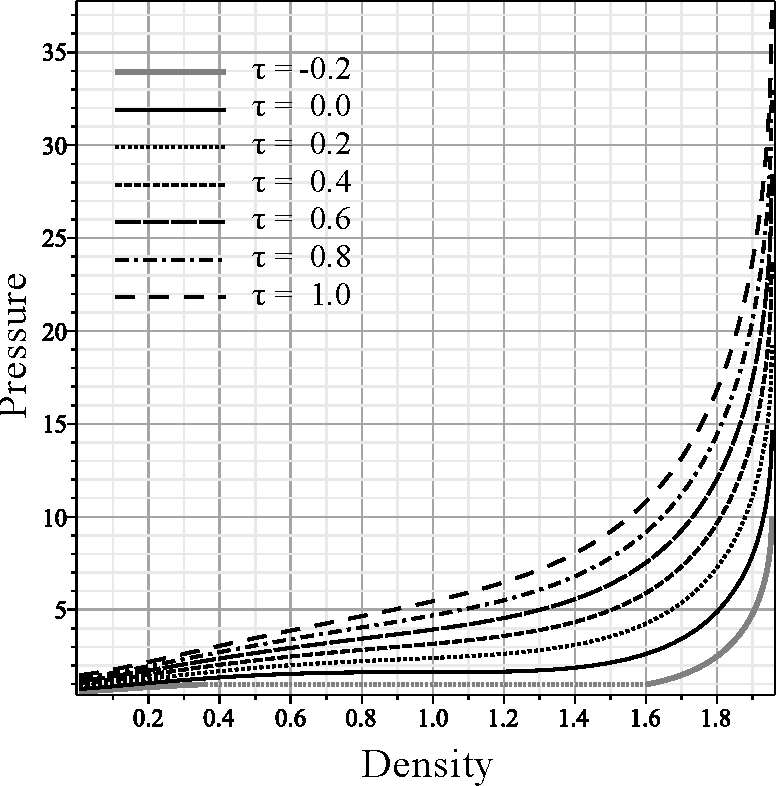
\includegraphics[width=0.446\textwidth]{f1a1.pdf} 
		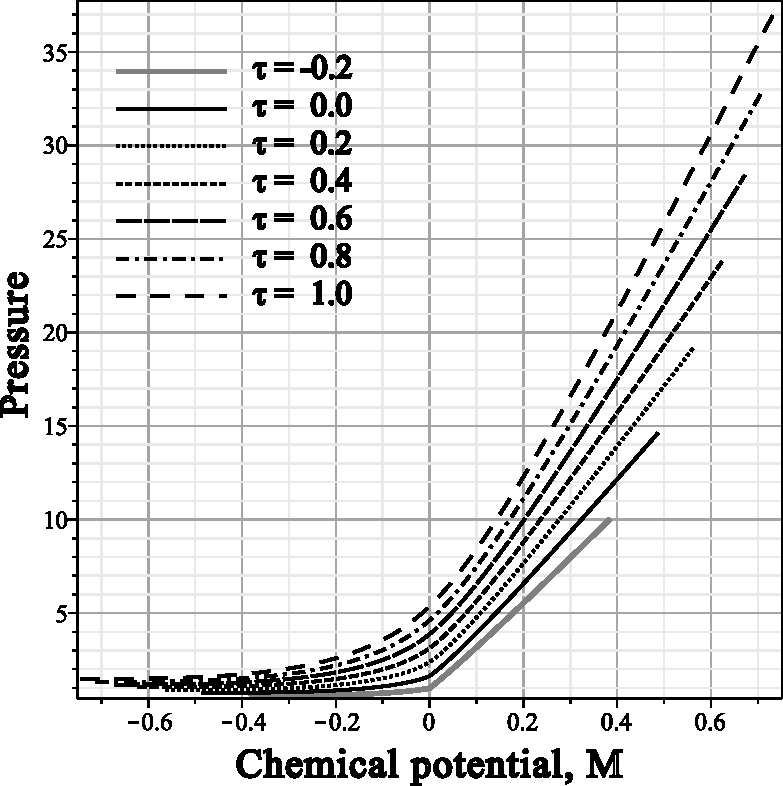
\includegraphics[width=0.45\textwidth]{f1b1.pdf} 
		\vskip-3mm\caption{Plots of isotherms of the pressure $P$ as a function of the density $\bar n$ (on the lefthand side) and a function of the effective chemical potential $M$ (on the righthand side) at $T \geq T_c$ represented by black lines. Thick grey lines on both figures correspond to isotherms of pressure at $T < T_c$ based on the results taken from~\cite{KozlovskiiDobush2020}. 
		}\label{fig1}
	\end{figure}
	
	\section{Thermodynamic response functions (coefficients)}
	
	\subsection{Isothermal compressibility}
	The isothermal compressibility is defined by
	\begin{equation}
		\label{def:isotherm_compres}
		K_T = -\frac{1}{V}\left(\frac{\partial V}{\partial P}\right)_{T,\langle N\rangle}
	\end{equation}
	Let us perform some transformations to rewrite the definition for $K_T$ into a form that is more suitable for the equation of state~\eqref{eq:eosMT}.
	\begin{eqnarray*}
		K_T & = & - \frac{1}{V}\left(\frac{\partial V}{\partial P}\right)_{T,\langle N\rangle}
		\\
		& = & -\rho \left(\frac{\partial \left(\frac{1}{\rho}\right)}{\partial P}\right)_{T,\langle N\rangle}
		\\
		& = & \frac{1}{\rho} \left(\frac{\partial \rho}{\partial P} \right)_{T,\langle N\rangle}
		\\
		& = & \frac{1}{\rho} \frac{\left(\partial \rho / \partial \mu\right)_{T,\langle N\rangle}}
		{\left(\partial P / \partial \mu\right)_{T,\langle N\rangle}},
	\end{eqnarray*}
	where $\rho = \langle N \rangle / V$ is the particle number density.
	Applying the Gibbs--Duhem equation at $T = const$, one has
	\begin{equation*}
		{\rm d} P = \rho {\rm d} \mu,
	\end{equation*}
	or
	\begin{equation}
		\label{eq:rho_dpdm}
		\rho = \left(\frac{\partial P}{\partial \mu}\right)_T.
	\end{equation}
	Substituting this into the last expression for $K_T$, one gets
	\begin{equation}
		K_T = \frac{1}{\rho^2} \left(\frac{\partial \rho}{\partial \mu}\right)_{T,\langle N\rangle}
	\end{equation}
	Finally, from~\eqref{eq:rho_dpdm} it follows that
	\begin{equation}
		\left(\frac{\partial \rho}{\partial \mu}\right)_T = \left(\frac{\partial^2 P}{\partial \mu^2}\right)_T
	\end{equation}
	and ultimately we arrive at the very useful expression for the isothermal compressibility
	\begin{equation}
		K_T = \frac{1}{\rho^2} \left(\frac{\partial^2 P}{\partial \mu^2}\right)_{T,\langle N\rangle}
	\end{equation}
	
	\begin{figure}[h!]
		\centering 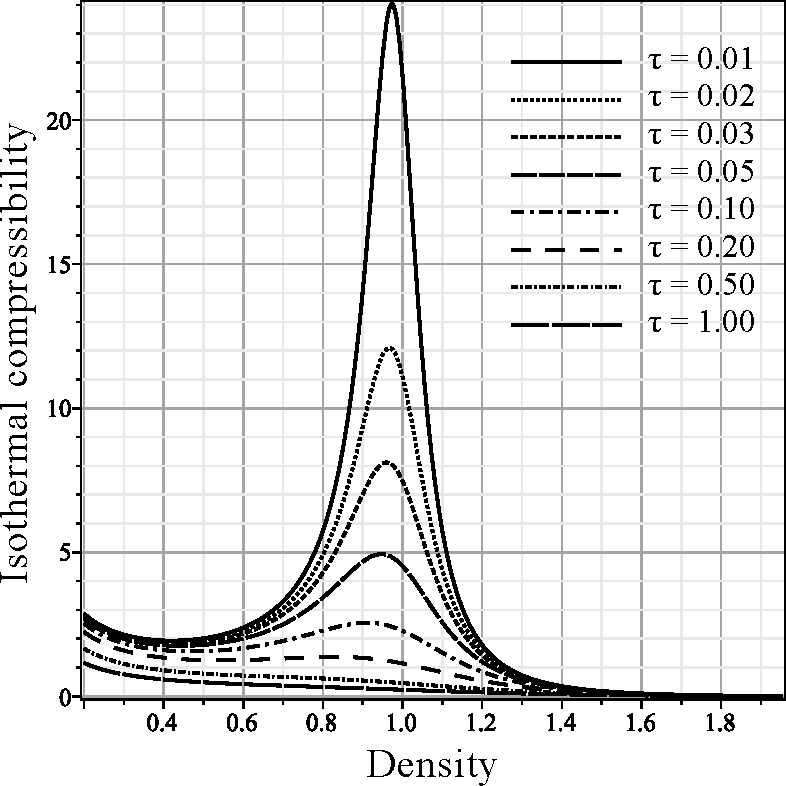
\includegraphics[width=0.5\textwidth]{f2a.pdf}
		\vskip-3mm\caption{The isothermal compressibility $K_T$ as a function of the density $\bar n$ at different values of reduced temperature $\tau > 0$ ($T > T_c$). 
		}\label{fig2a}
	\end{figure}
	
	\begin{figure}[h!]
		\centering 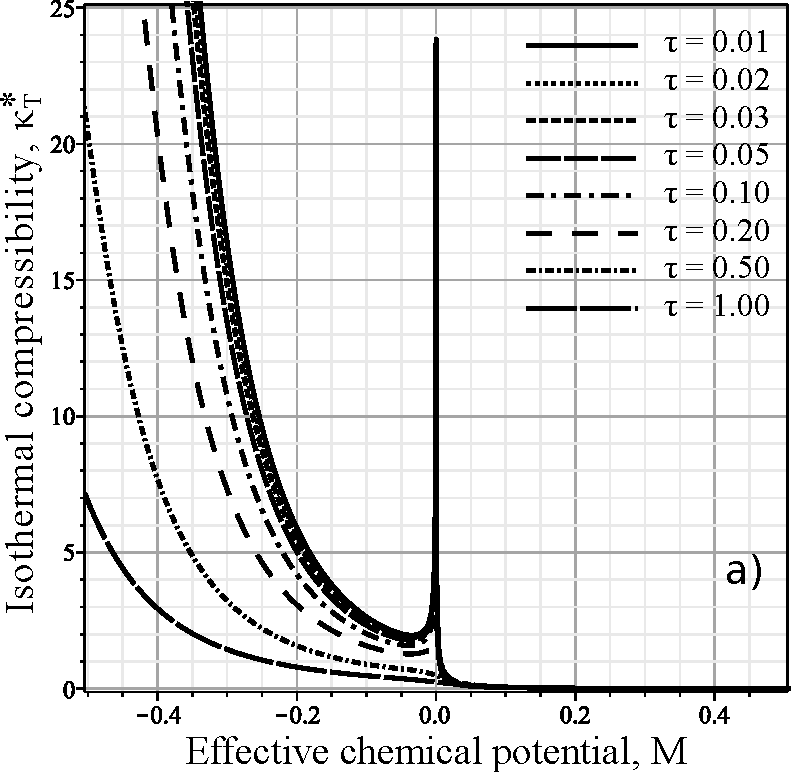
\includegraphics[width=0.45\textwidth]{f2b.pdf}
		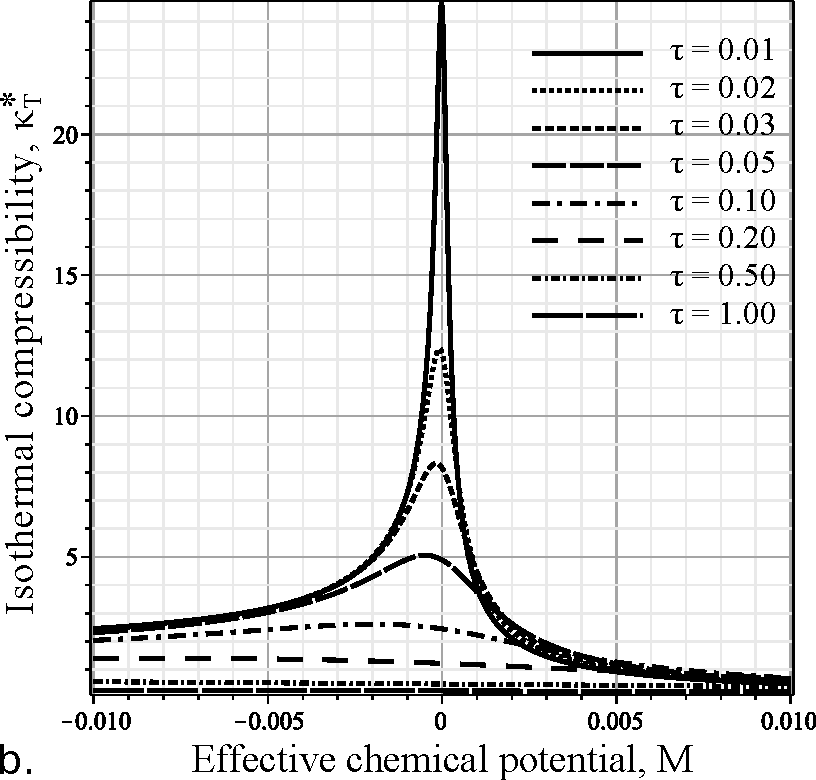
\includegraphics[width=0.475\textwidth]{f2c.pdf}
		\vskip-3mm\caption{The isothermal compressibility $K_T$ as a function of the effective chemical potential $M$ for different temperatures $\tau = (T - T_c)/T_c$ at $T > T_c$. The two figures differ in the scale of $M$. The left-hand-side figure covers a wider range of $M$, while the right-hand-side one focuses on a range of $M$ around its critical value $0$.
		}\label{fig2b}
	\end{figure}
	
	\subsection{Thermal pressure coefficient}
	The thermal pressure coefficient is defined by
	\begin{equation}
		\label{def:therm_pres_coef}
		\beta_V = \left( \frac{\partial P}{\partial T} \right)_{V,\langle N \rangle}
	\end{equation}
	
	\begin{figure}[h!]
		\centering 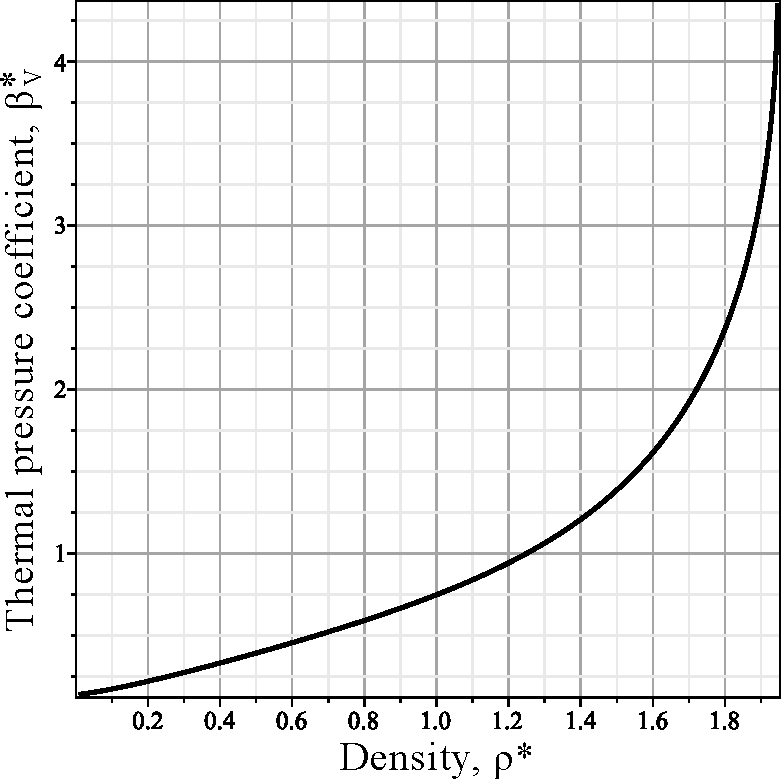
\includegraphics[width=0.5\textwidth]{f3a.pdf}
		\vskip-3mm\caption{The thermal pressure coefficient $\beta_V$ as a function of the density $\bar n$ at different values of relative temperature $\tau > 0$ ($T > T_c$). 
		}\label{fig3a}
	\end{figure}
	\begin{figure}[h!]
		\centering 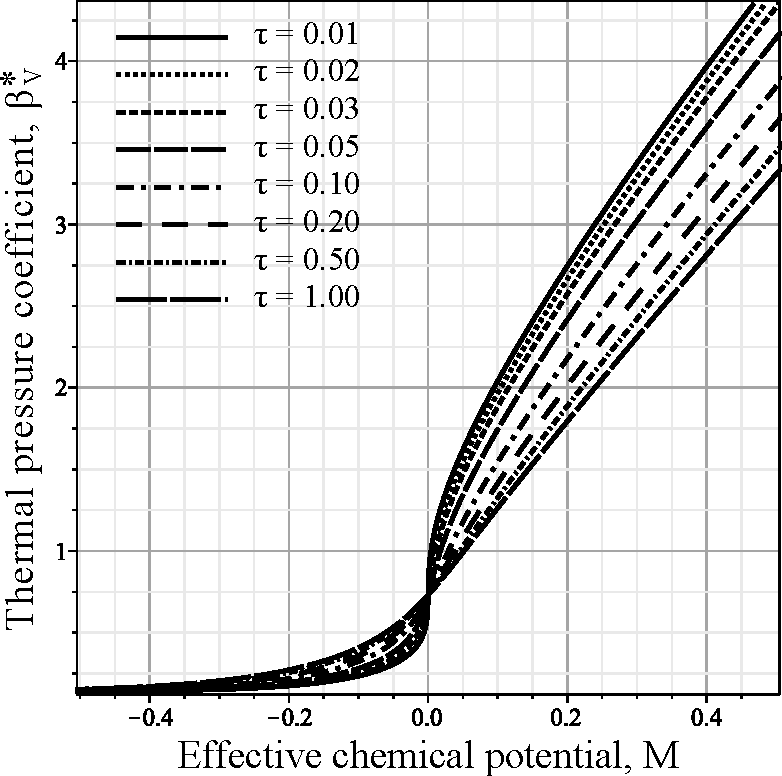
\includegraphics[width=0.5\textwidth]{f3b.pdf}
		\vskip-3mm\caption{The thermal pressure coefficient $\beta_V$ as a function of the effective chemical potential $M$ at different values of relative temperature $\tau > 0$ ($T > T_c$). 
		}\label{fig3b}
	\end{figure}
	\begin{figure}[h!]
		\centering 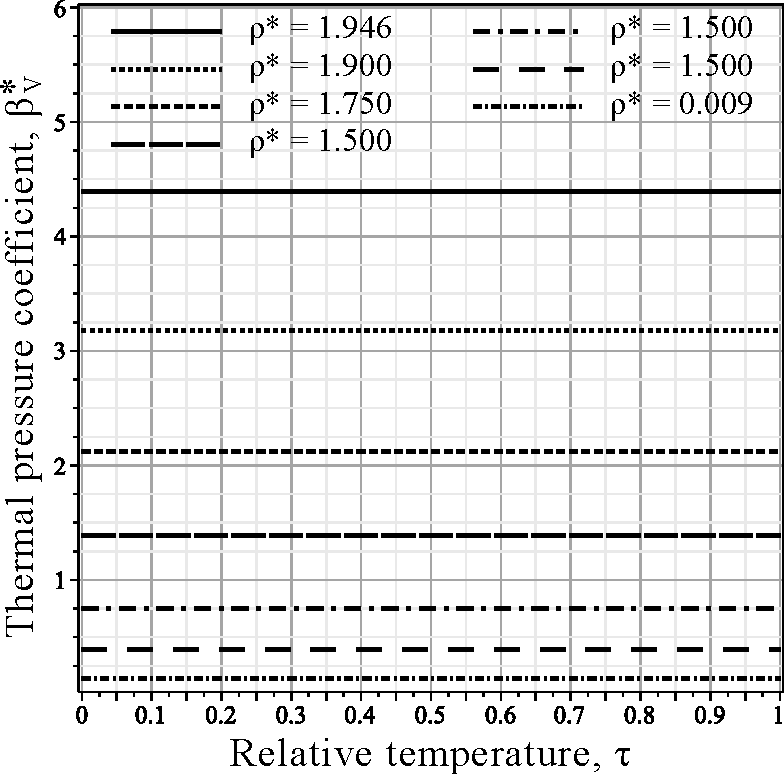
\includegraphics[width=0.5\textwidth]{f3c.pdf}
		\vskip-3mm\caption{The thermal pressure coefficient $\beta_V$ as a function of the relative temperature $\tau$ at different values of the density $\eta$. 
		}\label{fig3c}
	\end{figure}
	
	\subsection{Thermal expansion coefficient}
	The thermal expansion coefficient is defined by
	\begin{equation}
		\alpha_P = \frac{1}{V}\left(\frac{\partial V}{\partial T}\right)_{P,\langle N\rangle}
	\end{equation}
	
	\begin{figure}[h!]
		\centering 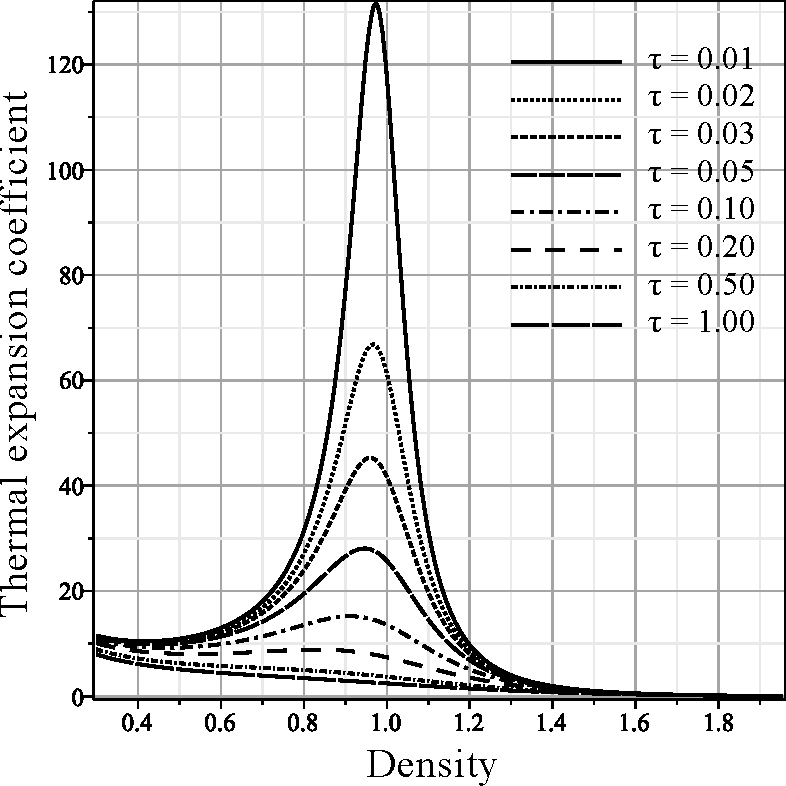
\includegraphics[width=0.5\textwidth]{f4a.pdf}
		\vskip-3mm\caption{The thermal expansion coefficient $\alpha_P$ as a function of the density $\bar n$ at different values of relative temperature $\tau > 0$ ($T > T_c$). 
		}\label{fig4a}
	\end{figure}
	
		\begin{figure}[h!]
		\centering 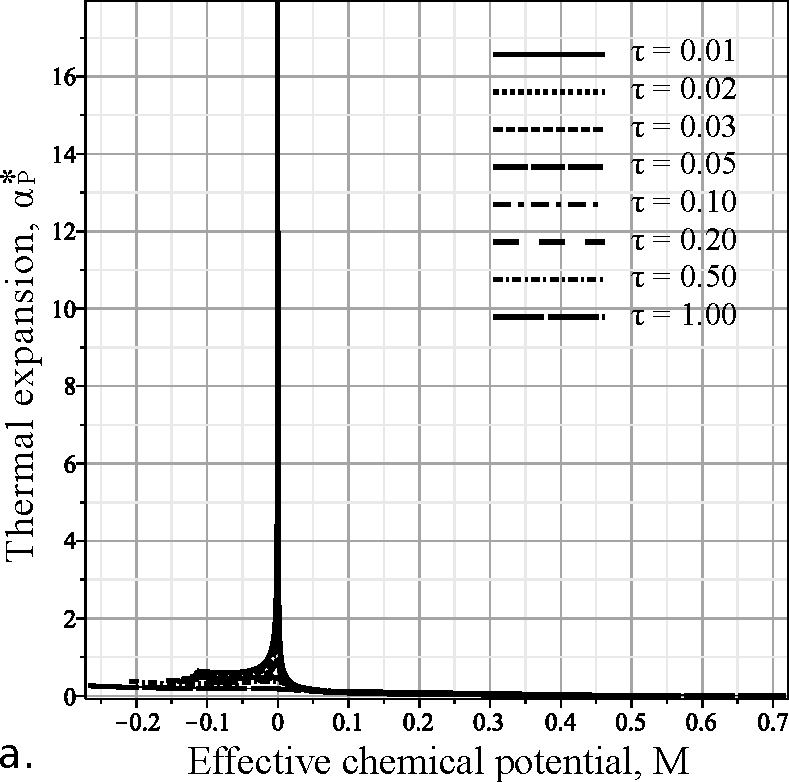
\includegraphics[width=0.45\textwidth]{f4b.pdf}
		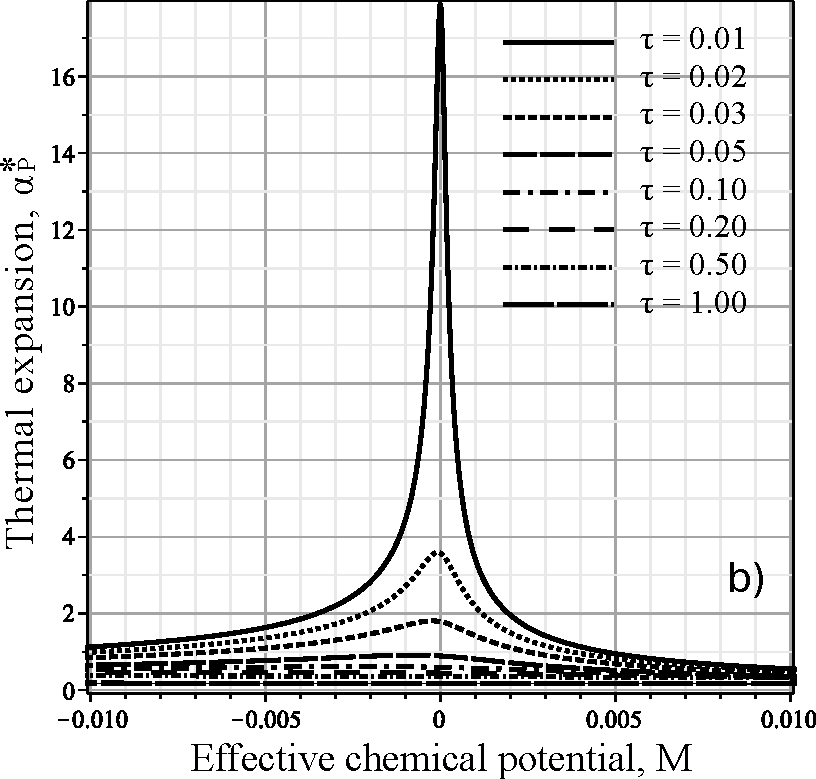
\includegraphics[width=0.475\textwidth]{f4c.pdf}
		\vskip-3mm\caption{The thermal expansion coefficient $\alpha_P$ as a function of the effective chemical potential $M$ for different temperatures $\tau = (T - T_c)/T_c$ at $T > T_c$. The two figures differ in the scale of $M$. The left-hand-side figure covers a wider range of $M$, while the right-hand-side one focuses on a range of $M$ around its critical value $0$.
		}\label{fig4b}
	\end{figure}
	
	\newpage 
	
	\section{Conclusions}
	Thermodynamic response functions, namely the isothermal compressibility, the thermal pressure coefficient, and the thermal expansion coefficient, are calculated for a many-particle system interacting through a modified Morse potential.
	
	%\bibliographystyle{cmpj} % still looking for the best style
	\bibliographystyle{elsarticle-num}
	%\bibliographystyle{unsrturl}
	%\bibliography{fluids_general,fluids_cv} % BibTeX / BibLaTeX should be used
	\bibliography{extracted}
	
\end{document}